\section{积分的基本性质}
\label{sec:integral-properties}

上一节的积分由上确界定义，单调性可以直接读出，但加法却不明显：$f$下方的简单函数与$g$下方的简单函数相加，得到的只是$f+g$下方的一部分候选，不能立即推出$\int(f+g)=\int f+\int g$。本节先证明非负函数的递增逼近可以与积分交换，借此把简单函数的运算规则传递到一般非负函数；随后分别处理可正可负的实值函数与复值函数，最后把这些规则推广到上一节已经定义的有符号测度积分。

\subsection{单调收敛定理}
\label{sec:integral-mct}

\paragraph{定理与证明}
定义~\ref{def:integral-nonnegative}没有指定逼近列。若一列非负函数从下方递增地逼近$f$，它们的积分是否趋于$\int f$？下面的定理给出肯定回答，并允许两边同时为$+\infty$。

\begin{theorem}[单调收敛定理]
\label{thm:integral-monotone-convergence}
设$f_1,f_2,\dots:X\to[0,+\infty]$可测，且$f_1\le f_2\le\cdots$处处成立，令$f=\lim_nf_n=\sup_nf_n$。则$f$可测，并且
\[
 \lim_{n\to\infty}\int_Xf_n\,\mathrm d\mu=\int_Xf\,\mathrm d\mu,
\]
两边可以同时等于$+\infty$。这一结论称为\term{单调收敛定理}（monotone convergence theorem）。
\end{theorem}

\begin{proof}
$f$是可数个可测函数的上确界，由定理~\ref{thm:measure-limits}可测。由引理~\ref{lem:integral-nonnegative-basic}第1条，$\int f_n$关于$n$递增，且每项不超过$\int f$；记极限为$L\in[0,+\infty]$，则$L\le\int f$。

反向不等式需要说明$f$下方的每个简单函数都被$f_n$的积分最终超过。固定非负简单函数$s\le f$与常数$c\in(0,1)$，令
\[
 E_n=\{x:f_n(x)\ge c\,s(x)\}.
\]
把$s$写成分割上的表示$s=\sum_ic_i\mathbf 1_{A_i}$，则$E_n=\bigcup_i\bigl(A_i\cap\{f_n\ge cc_i\}\bigr)$是阈值集合与可测集之交的有限并，可测；并且由$f_n$递增知$E_1\subseteq E_2\subseteq\cdots$。这列集合填满$X$：若$s(x)=0$，则$x\in E_1$；若$s(x)>0$，则$cs(x)<s(x)\le f(x)=\sup_nf_n(x)$，故某个$f_n(x)\ge cs(x)$。在$E_n$上$f_n\ge cs$，因此
\[
 \int_Xf_n\,\mathrm d\mu\ge\int_Xf_n\mathbf 1_{E_n}\,\mathrm d\mu\ge c\int_{E_n}s\,\mathrm d\mu.
\]

由引理~\ref{lem:integral-simple-properties}第4条，$E\mapsto\int_Es\,\mathrm d\mu$是测度；由测度的从下连续性（定理~\ref{thm:measure-basic-properties}），$\int_{E_n}s\to\int_Xs$。令$n\to\infty$得$L\ge c\int_Xs$。再令$c\uparrow1$得$L\ge\int s$，对$f$下方的全部$s$取上确界，得$L\ge\int f$。
\end{proof}

缩小因子$c<1$是证明的关键。若直接取$E_n=\{f_n\ge s\}$，在$f(x)=s(x)$而每个$f_n(x)<f(x)$的点上，$x$永远不进入$E_n$，集合列就不能填满$X$。乘以$c$留出一点余量，使严格不等式$cs(x)<f(x)$能被递增列在有限步内越过。图~\ref{fig:integral-monotone-convergence-sets}在$[0,1]$上取$f_n(x)=x^{1/n}$，它递增到$f=\mathbf 1_{(0,1]}$；取$s=0.8\cdot\mathbf 1_{(0,1]}$、$c=0.9$，集合$E_n=[0.72^n,1]$随$n$向左扩张，左端点依次为$0.72$、$0.5184$、$0.2687$（$n=1,2,4$），最终覆盖$(0,1]$。

\begin{figure}[!htbp]
 \centering
 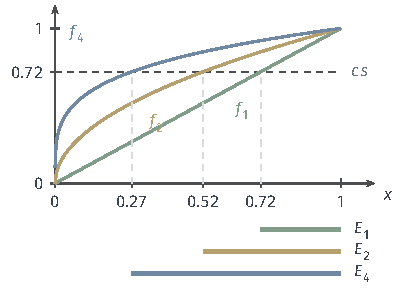
\includegraphics[width=68.273mm]{figures/02-abstract-mathematics/01-metric-and-measure/tikz/c3-monotone-convergence-sets/figure.pdf}
 \caption{单调收敛定理证明中的集合$E_n=\{f_n\ge cs\}$。$f_n(x)=x^{1/n}$（$n=1,2,4$）在$[0,1]$上递增到$\mathbf 1_{(0,1]}$；取$s=0.8\cdot\mathbf 1_{(0,1]}$、$c=0.9$，虚线为高度$cs=0.72$。下方三条线段是$E_n=[0.72^n,1]$，它们递增并逐步覆盖$(0,1]$。}
 \label{fig:integral-monotone-convergence-sets}
\end{figure}

定理只要求逐点递增与非负，不要求$f_n$或$f$可积。若递增与收敛只在零测集外成立，把各个零测例外合并为一个零测集$N$（可数个零测集之并仍为零测集），在$N$外应用定理于$f_n\mathbf 1_{X\setminus N}$，再由引理~\ref{lem:integral-nonnegative-basic}第3条知积分不受影响；这里需要$f$本身可测，在完备空间上这一点自动成立。

\paragraph{与简单函数逼近的衔接}
把定理用于引理~\ref{lem:integral-simple-approx}构造的$s_n\uparrow f$，立即得到
\[
 \int_Xf\,\mathrm d\mu=\lim_{n\to\infty}\int_Xs_n\,\mathrm d\mu.
\]
任何从下方递增逼近$f$的简单函数列都给出同一个极限，它就是定义中的上确界。这一结论使简单函数的有限运算能够传递到一般非负函数，下一小节正是这样做的。单调收敛定理在逐项求和、递增区域等计算中的使用，集中在第~\ref{sec:integral-limits-monotone}小节，后文不再重复证明。

\subsection{非负积分的运算性质}
\label{sec:integral-nonnegative-rules}

\paragraph{加法与数乘}
有了单调收敛定理，加法只需在逼近列上验证。

\begin{theorem}[非负积分的线性]
\label{thm:integral-nonnegative-linear}
设$f,g:X\to[0,+\infty]$可测，$a,b\in[0,+\infty)$。则
\[
 \int_X(af+bg)\,\mathrm d\mu=a\int_Xf\,\mathrm d\mu+b\int_Xg\,\mathrm d\mu.
\]
\end{theorem}

\begin{proof}
取引理~\ref{lem:integral-simple-approx}中的简单函数$s_n\uparrow f$、$t_n\uparrow g$。则$as_n+bt_n$是非负简单函数，逐点递增到$af+bg$（在$f$或$g$取$+\infty$的点上，按$[0,+\infty]$中的运算理解，且$0\cdot(+\infty)=0$）。由引理~\ref{lem:integral-simple-properties}第2条，$\int(as_n+bt_n)=a\int s_n+b\int t_n$。对两边令$n\to\infty$，三次应用单调收敛定理即得。
\end{proof}

这里只累计非负贡献，所有和都在$[0,+\infty]$中进行，不会出现无穷相减；当$a=0$而$\int f=+\infty$时，约定$0\cdot(+\infty)=0$与$af=0$的积分为零相符。例如在$[0,1]$上，由例~\ref{ex:integral-identity-on-unit}与$\int_{[0,1]}1\,\mathrm d\lambda=1$，得$\int_{[0,1]}(x+3)\,\mathrm dx=\tfrac12+3=\tfrac72$。

\paragraph{比较、区域与上下界}
单调性（引理~\ref{lem:integral-nonnegative-basic}第1条）与加法结合，就得到区域积分的常用规则。若$E,F\in\mathcal A$不交，则$f\mathbf 1_{E\cup F}=f\mathbf 1_E+f\mathbf 1_F$，由加法
\[
 \int_{E\cup F}f\,\mathrm d\mu=\int_Ef\,\mathrm d\mu+\int_Ff\,\mathrm d\mu,
\]
对有限个两两不交的区域同样成立。若$E\subseteq F$，则$f\mathbf 1_E\le f\mathbf 1_F$，故$\int_Ef\le\int_Ff$。若在$E$上$m\le f\le M$，则$m\mathbf 1_E\le f\mathbf 1_E\le M\mathbf 1_E$，得到上下界
\[
 m\,\mu(E)\le\int_Ef\,\mathrm d\mu\le M\,\mu(E).
\]

这些规则把分段给出的函数拆开计算。在$[0,2]$上令$f(x)=x$（$0\le x\le1$）、$f(x)=1$（$1<x\le2$），则$\int_{[0,2]}f=\int_{[0,1]}x\,\mathrm dx+\int_{(1,2]}1\,\mathrm dx=\tfrac12+1=\tfrac32$。又因为$0\le f\le1$，上下界给出$0\le\int_{[0,2]}f\le2$，与计算结果相容。对可数个不交区域的累计，需要交换积分与无限求和，第~\ref{sec:integral-limits-monotone}小节再用单调收敛定理处理。

\subsection{有符号积分的运算性质}
\label{sec:integral-signed-rules}

本小节的“有符号”指被积函数可正可负，测度本身仍然非负；复值情形沿用把函数拆成分量的办法。

\paragraph{可积性与线性}
先补全可积性的两个等价说法。对实值可测$f$，由定理~\ref{thm:integral-nonnegative-linear}，
\[
 \int_X|f|\,\mathrm d\mu=\int_Xf^+\,\mathrm d\mu+\int_Xf^-\,\mathrm d\mu,
\]
所以$f$可积当且仅当$\int f^+$与$\int f^-$都有限。对复值$f=u+\mathrm iv$，由$|f|\le|u|+|v|$与$|u|,|v|\le|f|$，并由单调性和加法，$f$可积当且仅当$u$与$v$都可积。可积的扩展实值函数几乎处处有限（引理~\ref{lem:integral-nonnegative-basic}第5条），把它在取无穷值的零测集上改为$0$不改变任何积分，因此下面只讨论取有限值的函数。

\begin{theorem}[积分的线性]
\label{thm:integral-linear}
设$f,g\in L^1(\mu)$为实值（或复值）函数，$a,b$为实数（或复数）。则$af+bg\in L^1(\mu)$，并且
\[
 \int_X(af+bg)\,\mathrm d\mu=a\int_Xf\,\mathrm d\mu+b\int_Xg\,\mathrm d\mu.
\]
\end{theorem}

\begin{proof}
可积性：$|af+bg|\le|a||f|+|b||g|$，由单调性与非负积分的线性，$\int|af+bg|\le|a|\int|f|+|b|\int|g|<+\infty$。

实值情形的加法。令$h=f+g$，则$h^+-h^-=f^+-f^-+g^+-g^-$，移项得
\[
 h^++f^-+g^-=h^-+f^++g^+.
\]
两边都是非负可测函数之和，由定理~\ref{thm:integral-nonnegative-linear}，$\int h^++\int f^-+\int g^-=\int h^-+\int f^++\int g^+$。六个积分都是有限数，移项即得$\int h=\int f+\int g$。

实值情形的数乘。若$a\ge0$，则$(af)^\pm=af^\pm$，由非负积分的数乘得$\int af=a\int f$；若$a<0$，则$(af)^+=|a|f^-$、$(af)^-=|a|f^+$，故$\int af=|a|\int f^--|a|\int f^+=a\int f$。

复值情形。设$f=u+\mathrm iv$，$a=\alpha+\mathrm i\beta$，则$af=(\alpha u-\beta v)+\mathrm i(\alpha v+\beta u)$。按定义与实值线性，
\[
 \begin{aligned}
  \int af&=\Bigl(\alpha\int u-\beta\int v\Bigr)+\mathrm i\Bigl(\alpha\int v+\beta\int u\Bigr)\\
  &=(\alpha+\mathrm i\beta)\Bigl(\int u+\mathrm i\int v\Bigr)=a\int f.
 \end{aligned}
\]
复值的加法逐个分量使用实值加法即可。
\end{proof}

线性也给出可积实值函数之间的比较：若$f\le g$且两者可积，则$g-f\ge0$，$\int g-\int f=\int(g-f)\ge0$。

\paragraph{绝对值估计}
积分的大小受绝对贡献的总量控制。实值函数可以利用大小比较，复值函数则需要先把积分结果旋转到实轴上。

\begin{theorem}[积分的绝对值估计]
\label{thm:integral-abs-bound}
对实值或复值$f\in L^1(\mu)$，有$\bigl|\int_Xf\,\mathrm d\mu\bigr|\le\int_X|f|\,\mathrm d\mu$。
\end{theorem}

\begin{proof}
实值情形：$-|f|\le f\le|f|$，由上面的比较得$-\int|f|\le\int f\le\int|f|$。复值情形：记$z=\int f$，若$z=0$无须证明。否则令$\alpha=\overline z/|z|$，则$|\alpha|=1$且$\alpha z=|z|$。由线性，$\int\alpha f=\alpha z=|z|$是实数，所以它等于实部的积分$\int\operatorname{Re}(\alpha f)$。由$\operatorname{Re}(\alpha f)\le|\alpha f|=|f|$与实值比较，$|z|=\int\operatorname{Re}(\alpha f)\le\int|f|$。
\end{proof}

估计中的等号对实值函数在$f$几乎处处不变号时成立，一般则严格：$f=\mathbf 1_{[0,1)}-\mathbf 1_{[1,2)}$在$[0,2]$上积分为$0$，而$\int|f|=2$。实值函数可以比较大小，复值函数没有大小顺序，只能使用这类模长估计。

\paragraph{用可积函数控制}
判断可积性时，往往不必计算$\int|f|$，只需找一个已知可积的上界。若$f$可测、$g\ge0$可积且$|f|\le g$几乎处处成立，则由引理~\ref{lem:integral-nonnegative-basic}第1、3条，$\int|f|\le\int g<+\infty$，$f$可积。特别地，在有限测度空间上，若$|f|\le M$，取$g=M$得$\int|f|\le M\mu(X)$：有界可测函数都可积。例如$f(x)=\sin(1/x)$在$(0,1]$上连续，因而Borel可测，又$|f|\le1$、$\lambda((0,1])=1$，所以它对$\lambda$可积，并且$\bigl|\int_{(0,1]}f\,\mathrm d\lambda\bigr|\le1$。这里不需要$f$在$0$附近有极限。

上面的规则都针对有限积分。对只是积分存在、可能取$\pm\infty$的实值函数，必须逐次检查表达式是否出现无定义的$\infty-\infty$，不能照搬线性。在$(\mathbb R,\lambda)$上取$f=\mathbf 1_{[0,+\infty)}$与$g=-\mathbf 1_{[0,+\infty)}$，两者的积分分别存在且等于$+\infty$与$-\infty$；$f+g=0$的积分是$0$，而$\int f+\int g=+\infty-\infty$没有意义。

\subsection{有符号测度积分的运算性质}
\label{sec:integral-signed-measure-rules}

\paragraph{测度相加时的积分}
第~\ref{sec:integral-signed-measure}小节把有符号测度的积分写成对Jordan正负部分的两个积分之差。要估计它的大小，需要知道对$|\eta|=\eta^++\eta^-$的积分怎样拆开。

\begin{lemma}[测度之和的积分]
\label{lem:integral-sum-of-measures}
设$\nu,\rho$是$(X,\mathcal A)$上的测度，$g\ge0$可测。则$\int_Xg\,\mathrm d(\nu+\rho)=\int_Xg\,\mathrm d\nu+\int_Xg\,\mathrm d\rho$。若$f$对$\nu+\rho$可积，则它对$\nu,\rho$都可积，上式对$f$也成立。
\end{lemma}

\begin{proof}
对非负简单函数$s=\sum_ic_i\mathbf 1_{A_i}$，$\int s\,\mathrm d(\nu+\rho)=\sum_ic_i(\nu(A_i)+\rho(A_i))=\int s\,\mathrm d\nu+\int s\,\mathrm d\rho$。取$s_n\uparrow g$，对三个测度分别应用单调收敛定理，得到非负情形。若$f$对$\nu+\rho$可积，由非负情形$\int|f|\,\mathrm d\nu\le\int|f|\,\mathrm d(\nu+\rho)<+\infty$，对$\rho$同理；把$f$拆成正负部（复值时再拆实部与虚部），逐项应用非负情形并相减。
\end{proof}

\begin{theorem}[有符号测度积分的运算规则]
\label{thm:integral-signed-measure-rules}
设$\eta$是有限有符号测度，$f,g$为实值或复值可测函数，且$\int|f|\,\mathrm d|\eta|$、$\int|g|\,\mathrm d|\eta|$有限。
\begin{enumerate}
 \item 对实数（或复数）$a,b$，$af+bg$满足同样的可积条件，且$\int(af+bg)\,\mathrm d\eta=a\int f\,\mathrm d\eta+b\int g\,\mathrm d\eta$。
 \item $\bigl|\int_Xf\,\mathrm d\eta\bigr|\le\int_X|f|\,\mathrm d|\eta|$。
\end{enumerate}
\end{theorem}

\begin{proof}
第1条：$|af+bg|\le|a||f|+|b||g|$，故$af+bg$对$|\eta|$可积，从而对$\eta^\pm$可积（第~\ref{sec:integral-signed-measure}小节）。对$\eta^+$与$\eta^-$分别使用定理~\ref{thm:integral-linear}，两式相减即得。

第2条：由定理~\ref{thm:integral-abs-bound}与引理~\ref{lem:integral-sum-of-measures}，
\[
 \begin{aligned}
  \Bigl|\int f\,\mathrm d\eta\Bigr|
  &\le\Bigl|\int f\,\mathrm d\eta^+\Bigr|+\Bigl|\int f\,\mathrm d\eta^-\Bigr|\\
  &\le\int|f|\,\mathrm d\eta^++\int|f|\,\mathrm d\eta^-=\int|f|\,\mathrm d|\eta|.
 \end{aligned}
\]
\end{proof}

估计可以取到等号。设$(P,N)$是$\eta$的Hahn分解（定理~\ref{thm:measure-hahn}），令$f=\mathbf 1_P-\mathbf 1_N$。由$\eta^+(N)=0$、$\eta^-(P)=0$，$\int f\,\mathrm d\eta=\eta^+(P)+\eta^-(N)=|\eta|(X)$，而$|f|=1$，右端也是$|\eta|(X)$。例~\ref{ex:integral-signed-measure-points}中$|-8|<12$，原因是$f$的符号没有与质量的符号配合：点$c$上质量为正而函数值为负。

\paragraph{保序性不再成立}
总变差控制累计的绝对贡献，但有符号测度积分没有一般的保序性。在$X=\{a,b\}$（$a\ne b$）上取$\eta=\delta_a-\delta_b$，则$0\le\mathbf 1_{\{b\}}$，而$\int\mathbf 1_{\{b\}}\,\mathrm d\eta=\eta(\{b\})=-1<0=\int0\,\mathrm d\eta$。非负测度的单调性来自“每块质量非负”；质量可以为负时，增大函数值反而可能减小积分。因此对有符号测度只能使用线性规则与总变差估计，比较大小时需要回到$\eta^+$与$\eta^-$分别处理。
